% Article type supporting font formatting
\documentclass[a4paper,12pt]{extarticle}

% Define .tex file encoding
\usepackage[utf8]{inputenc}

% Norwegian language support
%\usepackage[norsk]{babel}     

% Indent first paragraph in section
\usepackage{indentfirst}

% Allows mathbb in tex file
\usepackage{amsfonts} 

% Margin defining package
\usepackage{geometry}         
\geometry{a4paper
  ,margin=0.5in
}

% Math related tools and functions
\usepackage{mathtools} 

% For quotations
\usepackage{csquotes}

% Better bibliography 
\usepackage[round]{natbib}

% For use of graphics in document
\usepackage{graphicx}         

% Allows multi-line comments in tex file
\usepackage{verbatim} 

% Allows more control over tables
\usepackage{tabulary}

% Ads ul which allows line breaks while underlining text.
\usepackage{soul}      

% Allows math in tex file 
\usepackage{amsmath}          

% Allows math symbols in tex file
\usepackage{amssymb}          

% Allows use of physics shortcut functions
%\usepackage{physics}          

% Verbatim env with LaTeX commands
\usepackage{alltt}            

% Allows \begin{figure}[H]
\usepackage{float}

% Adds labeling list to the report
\usepackage{scrextend}
\addtokomafont{labelinglabel}{\ttfamily}

% Necessary for defining colours
\usepackage{xcolor}            
\definecolor{linkgreen}{rgb}{0,.5,0}
\definecolor{linkblue}{rgb}{0,0,.5}
\definecolor{linkred}{rgb}{.5,0,0}
\definecolor{blue}{rgb}{.13,.13,1}
\definecolor{green}{rgb}{0,.5,0}
\definecolor{red}{rgb}{.9,0,0}

% Hyperlinks in document
\usepackage{hyperref}  
\hypersetup{
  colorlinks=true,     % True for colored links
  linktoc=all,         % True for table of contents links
  linkcolor=linkblue,  % Colour for links
  urlcolor=linkgreen,  % Colour for URLs
  citecolor=linkred    % Colour for citations
}

% Listing package for code examples
\usepackage{listings}         
\lstset{
  language=C++,                % Set language to C++
  showspaces=false,            % Don't show space chars
  showtabs=false,              % Don't show tab chars
  breaklines=true,             % Break long lines of code
  showstringspaces=false,      % Don't show spaces in strings
  breakatwhitespace=true,      % Break at white space only
  commentstyle=\color{green},  % Set colour for comments
  keywordstyle=\color{blue},   % Set colours for keywords
  stringstyle=\color{red},     % Set colour for strings
  basicstyle=\ttfamily,        % Set basic style
  tabsize=2                    % Set tabsize
}

% Referencing, last for compatibility reasons
\usepackage[noabbrev]{cleveref}

% Makes matrices look square-ish
\renewcommand*{\arraystretch}{1.5}

% Allows number referencing the last page, used in footer
\usepackage{lastpage}

% Allows editing of header and footer data
\usepackage{fancyhdr}
\fancypagestyle{plain}{
  \fancyhf{}
  \renewcommand{\headrulewidth}{0pt}
  \rfoot[R]{\footnotesize Page \thepage\ of \pageref{LastPage}}
}
\pagestyle{fancy}
\fancyhf{}
\chead{\footnotesize P.A.Sundsbø, Reporttemplate for submission of student project in the master courses SMN6200, UiT Narvik 2018}
\rfoot{\footnotesize Page \thepage\ of \pageref{LastPage}}
\setlength{\headheight}{20pt}
\setlength{\footskip}{20pt}

% Allows editing of section headers
\usepackage{titlesec}
\titleformat*{\section}{\normalsize\bfseries}
\titleformat*{\subsection}{\normalsize\itshape\bfseries}
\titleformat*{\subsubsection}{\normalsize\bfseries}

%%%%%%%%%%%%%%%%%%%%%%%%%%%%%%%%%%%%%%%
%%      Title, Author, and Date      %%
%%%%%%%%%%%%%%%%%%%%%%%%%%%%%%%%%%%%%%%
\title{Report template for submission of student project in the master course SMN6200}
\author{P.A.Sundsbø}
\date{\parbox{\linewidth}{\centering
    \today\endgraf\bigskip
    \textit{\small UiT - The Arctic University of Norway, P.O. Box 385, N-8505 Narvik, Norway}
}}
\providecommand{\keywords}[1]{\textbf{\textit{\small{Keywords:}}} #1}

%%%%%%%%%%%%%%%%%%%%%%%%%%%%%%%%%%%%%%%
%%           Start document          %%
%%%%%%%%%%%%%%%%%%%%%%%%%%%%%%%%%%%%%%%
\begin{document}
  
%%%%%%%%%%%%%%%%%%%%%%%%%%%%%%%%%%%%%%%
%%   Create the main title section   %%
%%%%%%%%%%%%%%%%%%%%%%%%%%%%%%%%%%%%%%%
\maketitle

%%%%%%%%%%%%%%%%%%%%%%%%%%%%%%%%%%%%%%%
%%      Abstract for the report      %%
%%%%%%%%%%%%%%%%%%%%%%%%%%%%%%%%%%%%%%%
\begin{abstract} 
\noindent This document is a template for the report structure and text/content formatting for submission of the student project in the actual Master course. The reporting is based on an article structure similar to typical scientific journal requirements. The formatting must be identical to the one used in this description, i.e. Calibri, 11 pt size body text, 10 pt size figure text, justified alignment (body), single line spacing (body), top \& and bottom margins equal to 2.5 cm, left \& right equal to 2.0 cm etc. Beyond that, sizes and alignments must be according to the given document. Alternatively Latex fonts may be used. However, that applies to fonts only, layout and structure must be as described. The report must include the following parts; \textbf{Abstract, Introduction, Material \& Methods, Results \& Discussion, Conclusions, Acknowledgements, References and Appendices}.

The students must submit one pdf copy by e-mail, to the subject teacher. Maximal size of document is 10 pages excluding appendices. Problem/project and deadline for submission will be given in the beginning of the course. Prior to submitting your report/work, please follow strictly and carefully check the instructions given in this manuscript. Please note that the signature and student exam number must be included with the printed author names and affiliations. The language should be English and Norwegian.

\end{abstract}

\keywords{\small{Report Structure}; \small{Article Structure Description}; \small{Text Formatting}}

%%%%%%%%%%%%%%%%%%%%%%%%%%%%%%%%%%%%%%
%%  The main content of the report  %%
%%%%%%%%%%%%%%%%%%%%%%%%%%%%%%%%%%%%%%

\section{Introduction}
There are no universal report structures and formatting for writing e.q. academic papers, consultancy engineering reports or reports from analysis/laboratory activities. Academic journals have their individual structures and formatting, while company reporting may vary from close to research paper formats to only requiring a standard company front page. Using a fixed or defined structure like the one chosen for this course, might be very helpful for organizing and systematize your work and thoughts. Also, having a limited number of pages available automatically forces the writer(s) to concentrate on the most important material and information. The basic of the presented report structure in this article can be found in most of the published research articles, however the basic structure and methodology applies to reporting from consultancy engineering analysis/work as well.

An appropriate structure in the reporting improves and organizes the dissemination of results and knowledge. Formatting (fonts, sizes, alignments etc.) has developed to promote readability and understanding. As official language settings helps to preserve common writing in general, formatting helps to maintain certain readability standards. Imagine a world without any formatting standards for books, articles, magazines etc.

\subsection{About the abstract}
The abstract is a brief summary of the article/report and should briefly state the purpose of the analysis/work principal results and eventually major conclusions. In journals, company or report series etc. an abstract may act as a stand-alone entity and made to be presented separately. References etc. should therefore be avoided. For this student project, the abstract should not exceed 150 words.

\subsection{About the introduction}
The introduction should state the \ul{objectives} of the analysis/work and give the reader an adequate background. Why and where was the study undertaken? What was the purpose? Normally I state the extent, validity and/or limitations of the analysis/work, in the end of the introduction section. As an example, there might be uncertainties in the meteorological background data that forms the basis for a given local wind analysis. It is to be expected that the presented meteorological data is representative for the local wind conditions. The analysis will consequently not cover effects that occur with deviating wind conditions. Limitations connected to research method, the material available for the research or other such factors, may be located as a separate subdivision of the research discussion in the Material \& methods section.

\section{Material \& Methods}
\subsection{About the material \& methods part}
The presentation of the material and methods used in the actual work/analysis should be sufficient to be evaluated or reproduced. Methods or parts of methods that have already been published should be indicated by a reference. Do not include unnecessary details about commonly known or standardized methods that can be referred to. Limit the description to additional or unique applications and relevant modifications. Unlike the Abstract and the Introduction, the Material and methods part may be differently named and may also be a section of several chapters. Examples of commonly used chapters for this part are: Theory Modelling, Experimental apparatus and procedure, Experimental setup etc.

\subsection{About subdivision - numbered sections}
Subsections are to be numbered 1.1, 1.2, 1.3 etc. The report/article is limited in size so there is no need for further numbered subdivision into 1.1.1 etc. This numbering should also be used in the internal crossreferencing. Equations are numbered continuously by integer number regardless of sub chapters, and arranged as shown in the example below. Transport of drifting snow by suspension is modelled so that suspension approaches asymptotically a saturated transport rate given by:

\begin{equation}
  q_{suspension} = \frac{u(1)^{4.13}}{853119}
  \label{eq:FirstEquation}
\end{equation}

where u(10) is the air velocity at the height of 10m \citet{Tabler1990}.

Figures and tables are also numbered continuously, with text sizes and appearances as shown in the examples below. 

\begin{figure}[H]
  \centering
  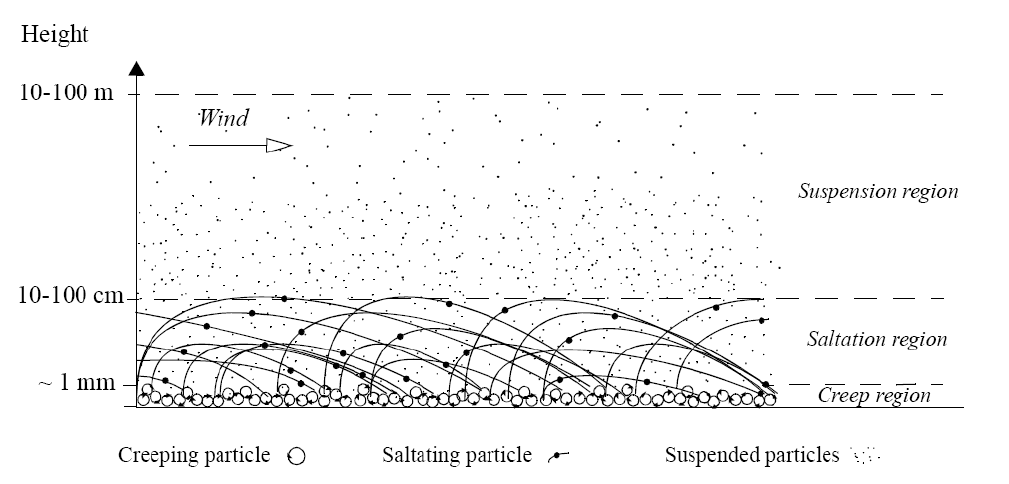
\includegraphics[width=0.8\textwidth]{SnowTransport.png}
  \caption{Illustration of the drifting snow transport regions above a horizontal snow surface. The transport regions are illustrated by the typical snow particle movements/behaviour \citet{Sundsbo1997}}
  \label{fig:SnowTransport}
\end{figure}

\begin{table}[H]
  \begin{tabulary}{\textwidth}{|L|L|}
    \hline
    Part in article structure & About function \& requirements \\\hline
    Abstract & Briefly states the purpose of the analysis/work principal results and eventually major conclusions. Should be enabled to be presented separately (fast track searches). \\ \hline
    1. Introduction & The introduction should state the objectives of the analysis/work and give the reader an adequate background. Possible include why and where was the study undertaken. \\ \hline
    2. Material \& Methods & Represents important documentation related to the work. Description \& references should be sufficient to evaluate or reproduced the work/analysis. \\ \hline
    3. Results \& Discussion  & This is normally the main section of the paper/report and results should be clear and concise. Limit the presentation of results to what is necessary for further discussion and conclusions. \\ \hline
    4. Conclusions  & The results \& discussions forms the basis for the main conclusion(s) and any conclusion must be presented as clear and concise as possible. \\ \hline
    Acknowledgements & As brief as possible. \\ \hline
    References & Check proper formatting and citations versus reference list. \\ \hline
    Appendices & Supplementary part, considered to be a necessity for the main target group of readers. \\\hline
  \end{tabulary}
  \caption{Basic structure for reporting in the actual course.}
  \label{tab:ReportStructure}
\end{table}

\subsection{Figure captions}
Ensure that each illustration has a caption that includes a brief title and description of the actual illustration. Text can also be included in the illustrations, e.g. on a photo, graph etc. Text in the text is useful for explaining symbols and abbreviations used. The caption text should be kept to a minimum. However, as a thumb rule the figure with caption should be sufficient to understand the figure/illustration without reading the surrounding body text.

\subsection{About References}
Use the suggested citation style which includes Author family name(s) and year of publication, hence (Author family name(s), year of publication). The reference list must then be arranged correspondingly according to family names of the corresponding or first author and year. In this way the reader does not necessary have to look back in the reference list to check the origin of the actual information or theory. Any citation in the text must refer to a reference in the reference list and visa versa. Example:

\begin{description}
    \item[Citation in the text:] \citet{Sundsbo1998}
    \item[Corresponding reference in Reference list:] \hfill \\ Sundsbø, P.-A. and Bang, B. (1998). International Snow Science Workshop, page 279–283.
\end{description}

For Web references, please use author/organization names, dates, reference to a source publication, etc., if available. This together with a full URL (Uniform Resource Locator). As a minimum, the full URL must be given. Web references can be included in the reference list or be listed separately after the reference list.

\begin{description}
  \item[Citation in the text:] \citet{FlowScienceInc2010}
  \item[Corresponding reference in Reference list:] \hfill \\ Flow Science Inc (2010). Flow 3d. http://www.flow3d.com/apps/index.html. Accesed on 2010-10-21.
\end{description}

\begin{description}
  \item[Citation in the text:] \citet{SINTEF2010}
  \item[Corresponding reference in Reference list]: \hfill \\ SINTEF (2010). The centre for renewable energy. http://www.sintef.no/Home/Environment/fornybar-energi. Accesed on 2010-10-25.
\end{description}

\begin{description}
  \item[Several citations from the same source:] \citet[a]{SINTEF2010}, using a, b, c etc.
\end{description}

\begin{description}
  \item[Several references on one citation:] (\citet{SINTEF2010}; \citet{FlowScienceInc2010})
\end{description}

\subsection{About the Appendices}
Appendices are to be located in the end of the document since this is considered as a supplementary part, however considered to be a necessity for the main target group of readers. If there is more than one appendix, they should be numbered as A, B, etc. Further numbering in the appendices must be related to the given appendix (\cref{eq:FirstEquation}, \cref{tab:ReportStructure}, \cref{fig:SnowTransport}, etc.). 

Source code may be located in the appendices or attached in digital format. Any programming parts that might be considered as real goodies may be located in the results section of the report. However, this depends highly on the nature of the project. In general, limit the attached data material to what is considered to be a necessity for the main target group for the particular work. Any attached digital video formats must be compatible with commonly used software.

\subsection{Reporting from a reading course, review of an engineering topic or State of the Art}
Engineers and researchers do regularly encounter problems or challenges that require an in depth study to gain more knowledge and understanding about a specific type of problem or solution methods. For a researcher this normally means reading articles describing the latest, related research results. Often this means investigating state of the art of the research area for a given topic. Writing of typical State of the art research articles normally requires a certain amount of international level research experience. An engineer must sometimes gather information to prepare for or to enable engineering solutions or analysis. This preparation may be for himself, for co-workers or to establish a decision background for costs/resources related to processes. 

An engineering student must always keep in mind the very purpose of doing such an investigation. Main objectives must always be clear and that must be reflected in the reporting. Students often ask themselves (and others) what to write in the conclusions. “We have been collecting a lot of material on the actual topic and arranged the results in a logical structure…., so what?’ Well, this is normally a result of the commonly used cut-and-paste-from-literature / Web-without-thinking-method. \ul{Please pay special attention to possible conclusions already from the start of the actual work or analyses}. In typical method investigations or in dept studies it is especially important always to maintain the awareness regarding the main objectives for doing the work. A good advice is regularly to look for possible solutions or conclusions to your questions.

\section{Results \& Discussion}
This is normally the main section of the paper/report and results should be clear and concise. Limit the presentation of results to what is necessary for further discussion and conclusions. Remaining material may alternatively be presented in the Appendices. For consultancy analysis the results must be sufficient to fulfil the task requirements and providing a solution to the problem/mission.

\ul{The discussion should supplement the results} by explaining, evaluating and exploring the significance of the results of the work/analysis. \textbf{It is not necessary to repeat or recreate all what we clearly should have seen from the results (illustrations, pictures, tables, graphs etc.)}. Illustrations with belonging text info should be self-explanatory. The discussions may be included in the Results part however the discussion may also be presented separately after.

\section{Conclusions}
The results and discussions forms the basis for the main conclusion(s) and any conclusion must be presented as clear and concise as possible. The conclusions are normally presented in a separate short Conclusions section (as in this description). However, Conclusions may be a subsection of a Discussion or Results and Discussion section.

The conclusions in an average student work/project are normally weak and often the weakest point of the report. \ul{Please pay special attention to possible conclusions already from the start of the actual work or analyses}. By always keeping an awareness regarding the main objectives for doing the work or making the analysis, the conclusions regarding whether you have achieved your goals or not, becomes clear.

As a student and later working with engineering analysis, research etc., always keep in mind that structuring your reporting also will increase the efficiency of the work itself and thereby improving your results.

Suggestions and recommendations for further work or analysis should be located in or immediately after the conclusions section. This since reflections about the further work naturally is the ‘final’ words from the author(s) to the reader and that these recommendations are normally founded on the conclusions. 

\section{Acknowledgements}
The author would like to thank his colleagues at the postgraduate studies at UiT The arctic university of Norway in Narvik for reading and commenting on this document (Providing language help, writing assistance or proof reading the article, etc.).

\section{References}
\begingroup
\def\section*#1{}
\bibliographystyle{apalike}
\bibliography{References}
\endgroup

\pagebreak
\appendix
\section{Appendix A. Example on research paper and consultancy report structure}
\begin{itemize}
  \item An appropriate structure on your reporting will often improve the structure of the actual work/analysis and thereby improving the final results.
  \item Most students/engineers develop a certain structure on a specific type work even if they think they do not.
\end{itemize}

The structure chosen for the reporting in this course consists of the following parts: Abstract, Introduction, Material \& Methods, Results \& Discussion, Conclusion, Acknowledgements, References and Appendices, reflects the basic within various types of scientific and engineering reporting. 

\subsection{Example on a research paper structure for publication in an international engineering journal:}
Beyers, J.H.M., Sundsbø, P.A. and Harms, T.M., 2004, Numerical simulation of three-dimensional, transient snow drifting around a cube, Journal of Wind Engineering and Industrial Aerodynamics, Volume 92, 725-747.

\begin{itemize}
  \item Abstract
  \item Nomenclature
  \item 1. Introduction
  \item 2. Numerical modelling (Material and Methods)
  \item 3. Experimental results (Results/Discussion)
  \item 4. Numerical results and discussion (Results/Discussion)
  \item 5. Conclusion
  \item Acknowledgements
  \item References
\end{itemize}

\subsection{Example on a consultancy report structure (large report, several issues):}
Sundsbø, P.A., 2004, Wind Chill Index- and snowdrift simulations/analysis on Hammerfest LNG Plant, WSB report 105-03 Rev 1, Commissioned by Tractebel Industry Engineering, Brussels.

\begin{itemize}
  \item Summary (Abstract)
  \item 1.0 Introduction
  \item 2.0 The Wind Chill Index (WCI) (Material and Methods)
  \item 3.0 Meteorological data – WCI (Material and Methods)
  \item 4.0 Snow drift conditions (Material and Methods)
  \item 5.0 Numerical model (Material and Methods)
  \item 6.0 Numerical simulations of WCI (Results/Discussion)
  \item 7.0 Numerical simulations of snowdrift (Results/Discussion)
  \item 8.0 Snow drift control (Results/Discussion)
  \item 9.0 Emergency escape ladder location (additional separate analysis)
  \item 10.0 Conclusions
  \item References
  \item Appendices (I-III, showing results from WCI \& snowdrift analysis)
\end{itemize}

Comments: Material related to modelling, programming, simulations and data collections may be presented in the Appendices. Do not include unnecessary data/info. Evaluate this carefully.

\pagebreak
\appendix
\section{Appendix B. Example on heading section for student project report}

\begin{figure}[H]
  \centering
  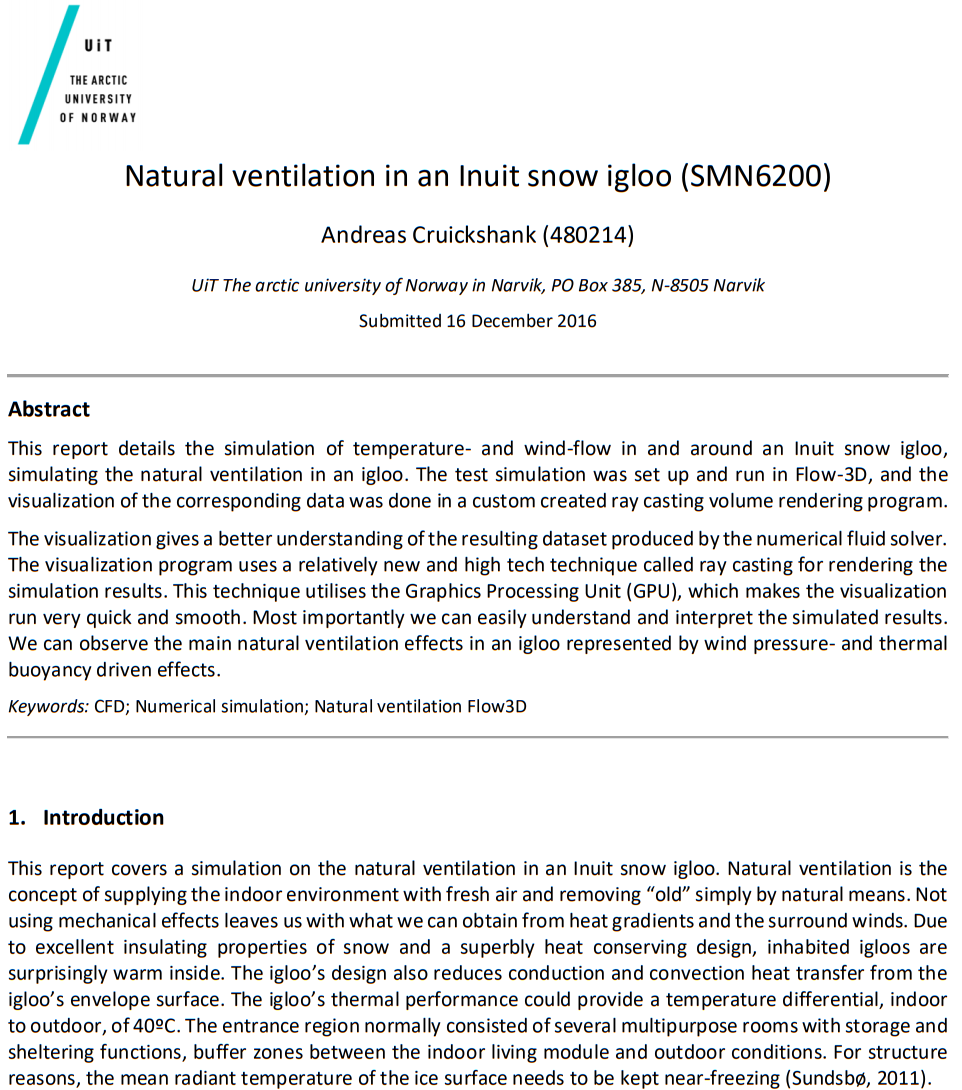
\includegraphics[width=\textwidth]{ProjectExample.png}
\end{figure}

\end{document} 